% Graphic for TeX using PGF
% Title: D:\Dokumente\GitHub\Bachelorarbeit\Arbeitstagebuch\src\04.07.2017-RPNTree-classdiagram.dia
% Creator: Dia v0.97.2
% CreationDate: Wed Jul 05 10:55:37 2017
% For: Timo Bergerbusch
% \usepackage{tikz}
% The following commands are not supported in PSTricks at present
% We define them conditionally, so when they are implemented,
% this pgf file will use them.
\ifx\du\undefined
  \newlength{\du}
\fi
\setlength{\du}{15\unitlength}
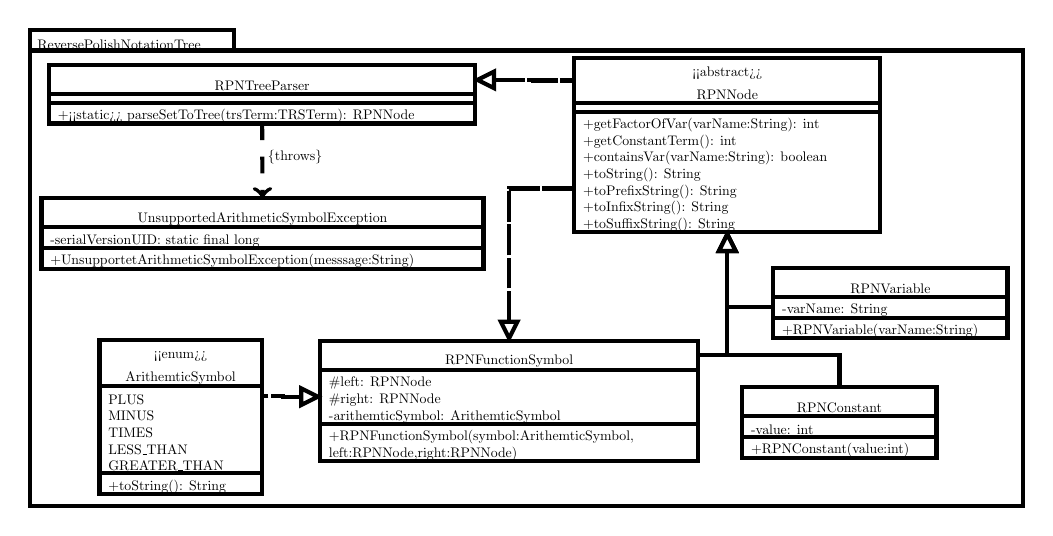
\begin{tikzpicture}[scale=0.5, every node/.style={scale=0.5}]
\pgftransformxscale{1.000000}
\pgftransformyscale{-1.000000}
\definecolor{dialinecolor}{rgb}{0.000000, 0.000000, 0.000000}
\pgfsetstrokecolor{dialinecolor}
\definecolor{dialinecolor}{rgb}{1.000000, 1.000000, 1.000000}
\pgfsetfillcolor{dialinecolor}
\pgfsetlinewidth{0.100000\du}
\pgfsetdash{}{0pt}
\definecolor{dialinecolor}{rgb}{1.000000, 1.000000, 1.000000}
\pgfsetfillcolor{dialinecolor}
\fill (-2.412994\du,34.090870\du)--(-2.412994\du,56.028781\du)--(45.422570\du,56.028781\du)--(45.422570\du,34.090870\du)--cycle;
\definecolor{dialinecolor}{rgb}{0.000000, 0.000000, 0.000000}
\pgfsetstrokecolor{dialinecolor}
\draw (-2.412994\du,34.090870\du)--(-2.412994\du,56.028781\du)--(45.422570\du,56.028781\du)--(45.422570\du,34.090870\du)--cycle;
\definecolor{dialinecolor}{rgb}{1.000000, 1.000000, 1.000000}
\pgfsetfillcolor{dialinecolor}
\fill (-2.412994\du,33.090870\du)--(-2.412994\du,34.090870\du)--(7.412006\du,34.090870\du)--(7.412006\du,33.090870\du)--cycle;
\definecolor{dialinecolor}{rgb}{0.000000, 0.000000, 0.000000}
\pgfsetstrokecolor{dialinecolor}
\draw (-2.412994\du,33.090870\du)--(-2.412994\du,34.090870\du)--(7.412006\du,34.090870\du)--(7.412006\du,33.090870\du)--cycle;
% setfont left to latex
\definecolor{dialinecolor}{rgb}{0.000000, 0.000000, 0.000000}
\pgfsetstrokecolor{dialinecolor}
\node[anchor=west] at (-2.312994\du,33.790870\du){ReversePolishNotationTree};
\pgfsetlinewidth{0.100000\du}
\pgfsetdash{}{0pt}
\definecolor{dialinecolor}{rgb}{1.000000, 1.000000, 1.000000}
\pgfsetfillcolor{dialinecolor}
\fill (23.823426\du,34.435422\du)--(23.823426\du,36.635422\du)--(38.568426\du,36.635422\du)--(38.568426\du,34.435422\du)--cycle;
\definecolor{dialinecolor}{rgb}{0.000000, 0.000000, 0.000000}
\pgfsetstrokecolor{dialinecolor}
\draw (23.823426\du,34.435422\du)--(23.823426\du,36.635422\du)--(38.568426\du,36.635422\du)--(38.568426\du,34.435422\du)--cycle;
% setfont left to latex
\definecolor{dialinecolor}{rgb}{0.000000, 0.000000, 0.000000}
\pgfsetstrokecolor{dialinecolor}
\node at (31.195926\du,35.195422\du){<<abstract>>};
% setfont left to latex
\definecolor{dialinecolor}{rgb}{0.000000, 0.000000, 0.000000}
\pgfsetstrokecolor{dialinecolor}
\node at (31.195926\du,36.235422\du){RPNNode};
\definecolor{dialinecolor}{rgb}{1.000000, 1.000000, 1.000000}
\pgfsetfillcolor{dialinecolor}
\fill (23.823426\du,36.635422\du)--(23.823426\du,37.035422\du)--(38.568426\du,37.035422\du)--(38.568426\du,36.635422\du)--cycle;
\definecolor{dialinecolor}{rgb}{0.000000, 0.000000, 0.000000}
\pgfsetstrokecolor{dialinecolor}
\draw (23.823426\du,36.635422\du)--(23.823426\du,37.035422\du)--(38.568426\du,37.035422\du)--(38.568426\du,36.635422\du)--cycle;
\definecolor{dialinecolor}{rgb}{1.000000, 1.000000, 1.000000}
\pgfsetfillcolor{dialinecolor}
\fill (23.823426\du,37.035422\du)--(23.823426\du,42.835422\du)--(38.568426\du,42.835422\du)--(38.568426\du,37.035422\du)--cycle;
\definecolor{dialinecolor}{rgb}{0.000000, 0.000000, 0.000000}
\pgfsetstrokecolor{dialinecolor}
\draw (23.823426\du,37.035422\du)--(23.823426\du,42.835422\du)--(38.568426\du,42.835422\du)--(38.568426\du,37.035422\du)--cycle;
% setfont left to latex
\definecolor{dialinecolor}{rgb}{0.000000, 0.000000, 0.000000}
\pgfsetstrokecolor{dialinecolor}
\node[anchor=west] at (23.973426\du,37.695422\du){+getFactorOfVar(varName:String): int};
% setfont left to latex
\definecolor{dialinecolor}{rgb}{0.000000, 0.000000, 0.000000}
\pgfsetstrokecolor{dialinecolor}
\node[anchor=west] at (23.973426\du,38.495422\du){+getConstantTerm(): int};
% setfont left to latex
\definecolor{dialinecolor}{rgb}{0.000000, 0.000000, 0.000000}
\pgfsetstrokecolor{dialinecolor}
\node[anchor=west] at (23.973426\du,39.295422\du){+containsVar(varName:String): boolean};
% setfont left to latex
\definecolor{dialinecolor}{rgb}{0.000000, 0.000000, 0.000000}
\pgfsetstrokecolor{dialinecolor}
\node[anchor=west] at (23.973426\du,40.095422\du){+toString(): String};
% setfont left to latex
\definecolor{dialinecolor}{rgb}{0.000000, 0.000000, 0.000000}
\pgfsetstrokecolor{dialinecolor}
\node[anchor=west] at (23.973426\du,40.895422\du){+toPrefixString(): String};
% setfont left to latex
\definecolor{dialinecolor}{rgb}{0.000000, 0.000000, 0.000000}
\pgfsetstrokecolor{dialinecolor}
\node[anchor=west] at (23.973426\du,41.695422\du){+toInfixString(): String};
% setfont left to latex
\definecolor{dialinecolor}{rgb}{0.000000, 0.000000, 0.000000}
\pgfsetstrokecolor{dialinecolor}
\node[anchor=west] at (23.973426\du,42.495422\du){+toSuffixString(): String};
\pgfsetlinewidth{0.100000\du}
\pgfsetdash{}{0pt}
\definecolor{dialinecolor}{rgb}{1.000000, 1.000000, 1.000000}
\pgfsetfillcolor{dialinecolor}
\fill (33.415475\du,44.559641\du)--(33.415475\du,45.959641\du)--(44.695475\du,45.959641\du)--(44.695475\du,44.559641\du)--cycle;
\definecolor{dialinecolor}{rgb}{0.000000, 0.000000, 0.000000}
\pgfsetstrokecolor{dialinecolor}
\draw (33.415475\du,44.559641\du)--(33.415475\du,45.959641\du)--(44.695475\du,45.959641\du)--(44.695475\du,44.559641\du)--cycle;
% setfont left to latex
\definecolor{dialinecolor}{rgb}{0.000000, 0.000000, 0.000000}
\pgfsetstrokecolor{dialinecolor}
\node at (39.055475\du,45.559641\du){RPNVariable};
\definecolor{dialinecolor}{rgb}{1.000000, 1.000000, 1.000000}
\pgfsetfillcolor{dialinecolor}
\fill (33.415475\du,45.959641\du)--(33.415475\du,46.959641\du)--(44.695475\du,46.959641\du)--(44.695475\du,45.959641\du)--cycle;
\definecolor{dialinecolor}{rgb}{0.000000, 0.000000, 0.000000}
\pgfsetstrokecolor{dialinecolor}
\draw (33.415475\du,45.959641\du)--(33.415475\du,46.959641\du)--(44.695475\du,46.959641\du)--(44.695475\du,45.959641\du)--cycle;
% setfont left to latex
\definecolor{dialinecolor}{rgb}{0.000000, 0.000000, 0.000000}
\pgfsetstrokecolor{dialinecolor}
\node[anchor=west] at (33.565475\du,46.619641\du){-varName: String};
\definecolor{dialinecolor}{rgb}{1.000000, 1.000000, 1.000000}
\pgfsetfillcolor{dialinecolor}
\fill (33.415475\du,46.959641\du)--(33.415475\du,47.959641\du)--(44.695475\du,47.959641\du)--(44.695475\du,46.959641\du)--cycle;
\definecolor{dialinecolor}{rgb}{0.000000, 0.000000, 0.000000}
\pgfsetstrokecolor{dialinecolor}
\draw (33.415475\du,46.959641\du)--(33.415475\du,47.959641\du)--(44.695475\du,47.959641\du)--(44.695475\du,46.959641\du)--cycle;
% setfont left to latex
\definecolor{dialinecolor}{rgb}{0.000000, 0.000000, 0.000000}
\pgfsetstrokecolor{dialinecolor}
\node[anchor=west] at (33.565475\du,47.619641\du){+RPNVariable(varName:String)};
\pgfsetlinewidth{0.100000\du}
\pgfsetdash{}{0pt}
\definecolor{dialinecolor}{rgb}{1.000000, 1.000000, 1.000000}
\pgfsetfillcolor{dialinecolor}
\fill (31.921154\du,50.304367\du)--(31.921154\du,51.704367\du)--(41.276154\du,51.704367\du)--(41.276154\du,50.304367\du)--cycle;
\definecolor{dialinecolor}{rgb}{0.000000, 0.000000, 0.000000}
\pgfsetstrokecolor{dialinecolor}
\draw (31.921154\du,50.304367\du)--(31.921154\du,51.704367\du)--(41.276154\du,51.704367\du)--(41.276154\du,50.304367\du)--cycle;
% setfont left to latex
\definecolor{dialinecolor}{rgb}{0.000000, 0.000000, 0.000000}
\pgfsetstrokecolor{dialinecolor}
\node at (36.598654\du,51.304367\du){RPNConstant};
\definecolor{dialinecolor}{rgb}{1.000000, 1.000000, 1.000000}
\pgfsetfillcolor{dialinecolor}
\fill (31.921154\du,51.704367\du)--(31.921154\du,52.704367\du)--(41.276154\du,52.704367\du)--(41.276154\du,51.704367\du)--cycle;
\definecolor{dialinecolor}{rgb}{0.000000, 0.000000, 0.000000}
\pgfsetstrokecolor{dialinecolor}
\draw (31.921154\du,51.704367\du)--(31.921154\du,52.704367\du)--(41.276154\du,52.704367\du)--(41.276154\du,51.704367\du)--cycle;
% setfont left to latex
\definecolor{dialinecolor}{rgb}{0.000000, 0.000000, 0.000000}
\pgfsetstrokecolor{dialinecolor}
\node[anchor=west] at (32.071154\du,52.364367\du){-value: int};
\definecolor{dialinecolor}{rgb}{1.000000, 1.000000, 1.000000}
\pgfsetfillcolor{dialinecolor}
\fill (31.921154\du,52.704367\du)--(31.921154\du,53.704367\du)--(41.276154\du,53.704367\du)--(41.276154\du,52.704367\du)--cycle;
\definecolor{dialinecolor}{rgb}{0.000000, 0.000000, 0.000000}
\pgfsetstrokecolor{dialinecolor}
\draw (31.921154\du,52.704367\du)--(31.921154\du,53.704367\du)--(41.276154\du,53.704367\du)--(41.276154\du,52.704367\du)--cycle;
% setfont left to latex
\definecolor{dialinecolor}{rgb}{0.000000, 0.000000, 0.000000}
\pgfsetstrokecolor{dialinecolor}
\node[anchor=west] at (32.071154\du,53.364367\du){+RPNConstant(value:int)};
\pgfsetlinewidth{0.100000\du}
\pgfsetdash{}{0pt}
\definecolor{dialinecolor}{rgb}{1.000000, 1.000000, 1.000000}
\pgfsetfillcolor{dialinecolor}
\fill (11.578208\du,48.068165\du)--(11.578208\du,49.468165\du)--(29.788208\du,49.468165\du)--(29.788208\du,48.068165\du)--cycle;
\definecolor{dialinecolor}{rgb}{0.000000, 0.000000, 0.000000}
\pgfsetstrokecolor{dialinecolor}
\draw (11.578208\du,48.068165\du)--(11.578208\du,49.468165\du)--(29.788208\du,49.468165\du)--(29.788208\du,48.068165\du)--cycle;
% setfont left to latex
\definecolor{dialinecolor}{rgb}{0.000000, 0.000000, 0.000000}
\pgfsetstrokecolor{dialinecolor}
\node at (20.683208\du,49.068165\du){RPNFunctionSymbol};
\definecolor{dialinecolor}{rgb}{1.000000, 1.000000, 1.000000}
\pgfsetfillcolor{dialinecolor}
\fill (11.578208\du,49.468165\du)--(11.578208\du,52.068165\du)--(29.788208\du,52.068165\du)--(29.788208\du,49.468165\du)--cycle;
\definecolor{dialinecolor}{rgb}{0.000000, 0.000000, 0.000000}
\pgfsetstrokecolor{dialinecolor}
\draw (11.578208\du,49.468165\du)--(11.578208\du,52.068165\du)--(29.788208\du,52.068165\du)--(29.788208\du,49.468165\du)--cycle;
% setfont left to latex
\definecolor{dialinecolor}{rgb}{0.000000, 0.000000, 0.000000}
\pgfsetstrokecolor{dialinecolor}
\node[anchor=west] at (11.728208\du,50.128165\du){\#left: RPNNode};
% setfont left to latex
\definecolor{dialinecolor}{rgb}{0.000000, 0.000000, 0.000000}
\pgfsetstrokecolor{dialinecolor}
\node[anchor=west] at (11.728208\du,50.928165\du){\#right: RPNNode};
% setfont left to latex
\definecolor{dialinecolor}{rgb}{0.000000, 0.000000, 0.000000}
\pgfsetstrokecolor{dialinecolor}
\node[anchor=west] at (11.728208\du,51.728165\du){-arithemticSymbol: ArithemticSymbol};
\definecolor{dialinecolor}{rgb}{1.000000, 1.000000, 1.000000}
\pgfsetfillcolor{dialinecolor}
\fill (11.578208\du,52.068165\du)--(11.578208\du,53.868165\du)--(29.788208\du,53.868165\du)--(29.788208\du,52.068165\du)--cycle;
\definecolor{dialinecolor}{rgb}{0.000000, 0.000000, 0.000000}
\pgfsetstrokecolor{dialinecolor}
\draw (11.578208\du,52.068165\du)--(11.578208\du,53.868165\du)--(29.788208\du,53.868165\du)--(29.788208\du,52.068165\du)--cycle;
% setfont left to latex
\definecolor{dialinecolor}{rgb}{0.000000, 0.000000, 0.000000}
\pgfsetstrokecolor{dialinecolor}
\node[anchor=west] at (11.728208\du,52.728165\du){+RPNFunctionSymbol(symbol:ArithemticSymbol,};
\definecolor{dialinecolor}{rgb}{0.000000, 0.000000, 0.000000}
\pgfsetstrokecolor{dialinecolor}
\node[anchor=west] at (11.728208\du,53.528165\du){                   left:RPNNode,right:RPNNode)};
\pgfsetlinewidth{0.100000\du}
\pgfsetdash{}{0pt}
\pgfsetmiterjoin
\pgfsetbuttcap
{
\definecolor{dialinecolor}{rgb}{0.000000, 0.000000, 0.000000}
\pgfsetfillcolor{dialinecolor}
% was here!!!
\definecolor{dialinecolor}{rgb}{0.000000, 0.000000, 0.000000}
\pgfsetstrokecolor{dialinecolor}
\draw (31.195926\du,42.835422\du)--(31.195926\du,46.459641\du)--(33.415475\du,46.459641\du);
}
\definecolor{dialinecolor}{rgb}{0.000000, 0.000000, 0.000000}
\pgfsetstrokecolor{dialinecolor}
\draw (31.195926\du,43.747226\du)--(31.195926\du,46.459641\du)--(33.415475\du,46.459641\du);
\pgfsetmiterjoin
\definecolor{dialinecolor}{rgb}{1.000000, 1.000000, 1.000000}
\pgfsetfillcolor{dialinecolor}
\fill (31.595926\du,43.747226\du)--(31.195926\du,42.947226\du)--(30.795926\du,43.747226\du)--cycle;
\pgfsetlinewidth{0.100000\du}
\pgfsetdash{}{0pt}
\pgfsetmiterjoin
\definecolor{dialinecolor}{rgb}{0.000000, 0.000000, 0.000000}
\pgfsetstrokecolor{dialinecolor}
\draw (31.595926\du,43.747226\du)--(31.195926\du,42.947226\du)--(30.795926\du,43.747226\du)--cycle;
% setfont left to latex
\pgfsetlinewidth{0.100000\du}
\pgfsetdash{}{0pt}
\pgfsetmiterjoin
\pgfsetbuttcap
{
\definecolor{dialinecolor}{rgb}{0.000000, 0.000000, 0.000000}
\pgfsetfillcolor{dialinecolor}
% was here!!!
\definecolor{dialinecolor}{rgb}{0.000000, 0.000000, 0.000000}
\pgfsetstrokecolor{dialinecolor}
\draw (31.195926\du,42.835422\du)--(31.195926\du,48.780402\du)--(36.598654\du,48.780402\du)--(36.598654\du,50.304367\du);
}
\definecolor{dialinecolor}{rgb}{0.000000, 0.000000, 0.000000}
\pgfsetstrokecolor{dialinecolor}
\draw (31.195926\du,43.747226\du)--(31.195926\du,48.780402\du)--(36.598654\du,48.780402\du)--(36.598654\du,50.304367\du);
\pgfsetmiterjoin
\definecolor{dialinecolor}{rgb}{1.000000, 1.000000, 1.000000}
\pgfsetfillcolor{dialinecolor}
\fill (31.595926\du,43.747226\du)--(31.195926\du,42.947226\du)--(30.795926\du,43.747226\du)--cycle;
\pgfsetlinewidth{0.100000\du}
\pgfsetdash{}{0pt}
\pgfsetmiterjoin
\definecolor{dialinecolor}{rgb}{0.000000, 0.000000, 0.000000}
\pgfsetstrokecolor{dialinecolor}
\draw (31.595926\du,43.747226\du)--(31.195926\du,42.947226\du)--(30.795926\du,43.747226\du)--cycle;
% setfont left to latex
\pgfsetlinewidth{0.100000\du}
\pgfsetdash{}{0pt}
\pgfsetmiterjoin
\pgfsetbuttcap
{
\definecolor{dialinecolor}{rgb}{0.000000, 0.000000, 0.000000}
\pgfsetfillcolor{dialinecolor}
% was here!!!
\definecolor{dialinecolor}{rgb}{0.000000, 0.000000, 0.000000}
\pgfsetstrokecolor{dialinecolor}
\draw (31.195926\du,42.835422\du)--(31.195926\du,48.768165\du)--(29.788208\du,48.768165\du);
}
\definecolor{dialinecolor}{rgb}{0.000000, 0.000000, 0.000000}
\pgfsetstrokecolor{dialinecolor}
\draw (31.195926\du,43.747226\du)--(31.195926\du,48.768165\du)--(29.788208\du,48.768165\du);
\pgfsetmiterjoin
\definecolor{dialinecolor}{rgb}{1.000000, 1.000000, 1.000000}
\pgfsetfillcolor{dialinecolor}
\fill (31.595926\du,43.747226\du)--(31.195926\du,42.947226\du)--(30.795926\du,43.747226\du)--cycle;
\pgfsetlinewidth{0.100000\du}
\pgfsetdash{}{0pt}
\pgfsetmiterjoin
\definecolor{dialinecolor}{rgb}{0.000000, 0.000000, 0.000000}
\pgfsetstrokecolor{dialinecolor}
\draw (31.595926\du,43.747226\du)--(31.195926\du,42.947226\du)--(30.795926\du,43.747226\du)--cycle;
% setfont left to latex
\pgfsetlinewidth{0.100000\du}
\pgfsetdash{}{0pt}
\definecolor{dialinecolor}{rgb}{1.000000, 1.000000, 1.000000}
\pgfsetfillcolor{dialinecolor}
\fill (0.948979\du,48.048596\du)--(0.948979\du,50.248596\du)--(8.763979\du,50.248596\du)--(8.763979\du,48.048596\du)--cycle;
\definecolor{dialinecolor}{rgb}{0.000000, 0.000000, 0.000000}
\pgfsetstrokecolor{dialinecolor}
\draw (0.948979\du,48.048596\du)--(0.948979\du,50.248596\du)--(8.763979\du,50.248596\du)--(8.763979\du,48.048596\du)--cycle;
% setfont left to latex
\definecolor{dialinecolor}{rgb}{0.000000, 0.000000, 0.000000}
\pgfsetstrokecolor{dialinecolor}
\node at (4.856479\du,48.808596\du){<<enum>>};
% setfont left to latex
\definecolor{dialinecolor}{rgb}{0.000000, 0.000000, 0.000000}
\pgfsetstrokecolor{dialinecolor}
\node at (4.856479\du,49.848596\du){ArithemticSymbol};
\definecolor{dialinecolor}{rgb}{1.000000, 1.000000, 1.000000}
\pgfsetfillcolor{dialinecolor}
\fill (0.948979\du,50.248596\du)--(0.948979\du,54.448596\du)--(8.763979\du,54.448596\du)--(8.763979\du,50.248596\du)--cycle;
\definecolor{dialinecolor}{rgb}{0.000000, 0.000000, 0.000000}
\pgfsetstrokecolor{dialinecolor}
\draw (0.948979\du,50.248596\du)--(0.948979\du,54.448596\du)--(8.763979\du,54.448596\du)--(8.763979\du,50.248596\du)--cycle;
% setfont left to latex
\definecolor{dialinecolor}{rgb}{0.000000, 0.000000, 0.000000}
\pgfsetstrokecolor{dialinecolor}
\node[anchor=west] at (1.098979\du,50.908596\du){ PLUS};
% setfont left to latex
\definecolor{dialinecolor}{rgb}{0.000000, 0.000000, 0.000000}
\pgfsetstrokecolor{dialinecolor}
\node[anchor=west] at (1.098979\du,51.708596\du){ MINUS};
% setfont left to latex
\definecolor{dialinecolor}{rgb}{0.000000, 0.000000, 0.000000}
\pgfsetstrokecolor{dialinecolor}
\node[anchor=west] at (1.098979\du,52.508596\du){ TIMES};
% setfont left to latex
\definecolor{dialinecolor}{rgb}{0.000000, 0.000000, 0.000000}
\pgfsetstrokecolor{dialinecolor}
\node[anchor=west] at (1.098979\du,53.308596\du){ LESS\_THAN};
% setfont left to latex
\definecolor{dialinecolor}{rgb}{0.000000, 0.000000, 0.000000}
\pgfsetstrokecolor{dialinecolor}
\node[anchor=west] at (1.098979\du,54.108596\du){ GREATER\_THAN};
\definecolor{dialinecolor}{rgb}{1.000000, 1.000000, 1.000000}
\pgfsetfillcolor{dialinecolor}
\fill (0.948979\du,54.448596\du)--(0.948979\du,55.448596\du)--(8.763979\du,55.448596\du)--(8.763979\du,54.448596\du)--cycle;
\definecolor{dialinecolor}{rgb}{0.000000, 0.000000, 0.000000}
\pgfsetstrokecolor{dialinecolor}
\draw (0.948979\du,54.448596\du)--(0.948979\du,55.448596\du)--(8.763979\du,55.448596\du)--(8.763979\du,54.448596\du)--cycle;
% setfont left to latex
\definecolor{dialinecolor}{rgb}{0.000000, 0.000000, 0.000000}
\pgfsetstrokecolor{dialinecolor}
\node[anchor=west] at (1.098979\du,55.108596\du){+toString(): String};
\pgfsetlinewidth{0.100000\du}
\pgfsetdash{{1.000000\du}{1.000000\du}}{0\du}
\pgfsetdash{{0.400000\du}{0.400000\du}}{0\du}
\pgfsetmiterjoin
\pgfsetbuttcap
{
\definecolor{dialinecolor}{rgb}{0.000000, 0.000000, 0.000000}
\pgfsetfillcolor{dialinecolor}
% was here!!!
\definecolor{dialinecolor}{rgb}{0.000000, 0.000000, 0.000000}
\pgfsetstrokecolor{dialinecolor}
\draw (11.578208\du,50.768165\du)--(9.771094\du,50.768165\du)--(9.771094\du,50.748596\du)--(8.763979\du,50.748596\du);
}
\definecolor{dialinecolor}{rgb}{0.000000, 0.000000, 0.000000}
\pgfsetstrokecolor{dialinecolor}
\draw (10.666405\du,50.768165\du)--(9.771094\du,50.768165\du)--(9.771094\du,50.748596\du)--(8.763979\du,50.748596\du);
\pgfsetmiterjoin
\definecolor{dialinecolor}{rgb}{1.000000, 1.000000, 1.000000}
\pgfsetfillcolor{dialinecolor}
\fill (10.666405\du,51.168165\du)--(11.466405\du,50.768165\du)--(10.666405\du,50.368165\du)--cycle;
\pgfsetlinewidth{0.100000\du}
\pgfsetdash{}{0pt}
\pgfsetmiterjoin
\definecolor{dialinecolor}{rgb}{0.000000, 0.000000, 0.000000}
\pgfsetstrokecolor{dialinecolor}
\draw (10.666405\du,51.168165\du)--(11.466405\du,50.768165\du)--(10.666405\du,50.368165\du)--cycle;
% setfont left to latex
\pgfsetlinewidth{0.100000\du}
\pgfsetdash{}{0pt}
\definecolor{dialinecolor}{rgb}{1.000000, 1.000000, 1.000000}
\pgfsetfillcolor{dialinecolor}
\fill (-1.476290\du,34.805480\du)--(-1.476290\du,36.205480\du)--(19.043710\du,36.205480\du)--(19.043710\du,34.805480\du)--cycle;
\definecolor{dialinecolor}{rgb}{0.000000, 0.000000, 0.000000}
\pgfsetstrokecolor{dialinecolor}
\draw (-1.476290\du,34.805480\du)--(-1.476290\du,36.205480\du)--(19.043710\du,36.205480\du)--(19.043710\du,34.805480\du)--cycle;
% setfont left to latex
\definecolor{dialinecolor}{rgb}{0.000000, 0.000000, 0.000000}
\pgfsetstrokecolor{dialinecolor}
\node at (8.783710\du,35.805480\du){RPNTreeParser};
\definecolor{dialinecolor}{rgb}{1.000000, 1.000000, 1.000000}
\pgfsetfillcolor{dialinecolor}
\fill (-1.476290\du,36.205480\du)--(-1.476290\du,36.605480\du)--(19.043710\du,36.605480\du)--(19.043710\du,36.205480\du)--cycle;
\definecolor{dialinecolor}{rgb}{0.000000, 0.000000, 0.000000}
\pgfsetstrokecolor{dialinecolor}
\draw (-1.476290\du,36.205480\du)--(-1.476290\du,36.605480\du)--(19.043710\du,36.605480\du)--(19.043710\du,36.205480\du)--cycle;
\definecolor{dialinecolor}{rgb}{1.000000, 1.000000, 1.000000}
\pgfsetfillcolor{dialinecolor}
\fill (-1.476290\du,36.605480\du)--(-1.476290\du,37.605480\du)--(19.043710\du,37.605480\du)--(19.043710\du,36.605480\du)--cycle;
\definecolor{dialinecolor}{rgb}{0.000000, 0.000000, 0.000000}
\pgfsetstrokecolor{dialinecolor}
\draw (-1.476290\du,36.605480\du)--(-1.476290\du,37.605480\du)--(19.043710\du,37.605480\du)--(19.043710\du,36.605480\du)--cycle;
% setfont left to latex
\definecolor{dialinecolor}{rgb}{0.000000, 0.000000, 0.000000}
\pgfsetstrokecolor{dialinecolor}
\node[anchor=west] at (-1.326290\du,37.265480\du){+<<static>> parseSetToTree(trsTerm:TRSTerm): RPNNode};
\pgfsetlinewidth{0.100000\du}
\pgfsetdash{}{0pt}
\definecolor{dialinecolor}{rgb}{1.000000, 1.000000, 1.000000}
\pgfsetfillcolor{dialinecolor}
\fill (-1.843383\du,41.197201\du)--(-1.843383\du,42.597201\du)--(19.446617\du,42.597201\du)--(19.446617\du,41.197201\du)--cycle;
\definecolor{dialinecolor}{rgb}{0.000000, 0.000000, 0.000000}
\pgfsetstrokecolor{dialinecolor}
\draw (-1.843383\du,41.197201\du)--(-1.843383\du,42.597201\du)--(19.446617\du,42.597201\du)--(19.446617\du,41.197201\du)--cycle;
% setfont left to latex
\definecolor{dialinecolor}{rgb}{0.000000, 0.000000, 0.000000}
\pgfsetstrokecolor{dialinecolor}
\node at (8.801617\du,42.197201\du){UnsupportedArithmeticSymbolException};
\definecolor{dialinecolor}{rgb}{1.000000, 1.000000, 1.000000}
\pgfsetfillcolor{dialinecolor}
\fill (-1.843383\du,42.597201\du)--(-1.843383\du,43.597201\du)--(19.446617\du,43.597201\du)--(19.446617\du,42.597201\du)--cycle;
\definecolor{dialinecolor}{rgb}{0.000000, 0.000000, 0.000000}
\pgfsetstrokecolor{dialinecolor}
\draw (-1.843383\du,42.597201\du)--(-1.843383\du,43.597201\du)--(19.446617\du,43.597201\du)--(19.446617\du,42.597201\du)--cycle;
% setfont left to latex
\definecolor{dialinecolor}{rgb}{0.000000, 0.000000, 0.000000}
\pgfsetstrokecolor{dialinecolor}
\node[anchor=west] at (-1.693383\du,43.257201\du){-serialVersionUID: static final long};
\definecolor{dialinecolor}{rgb}{1.000000, 1.000000, 1.000000}
\pgfsetfillcolor{dialinecolor}
\fill (-1.843383\du,43.597201\du)--(-1.843383\du,44.597201\du)--(19.446617\du,44.597201\du)--(19.446617\du,43.597201\du)--cycle;
\definecolor{dialinecolor}{rgb}{0.000000, 0.000000, 0.000000}
\pgfsetstrokecolor{dialinecolor}
\draw (-1.843383\du,43.597201\du)--(-1.843383\du,44.597201\du)--(19.446617\du,44.597201\du)--(19.446617\du,43.597201\du)--cycle;
% setfont left to latex
\definecolor{dialinecolor}{rgb}{0.000000, 0.000000, 0.000000}
\pgfsetstrokecolor{dialinecolor}
\node[anchor=west] at (-1.693383\du,44.257201\du){+UnsupportetArithmeticSymbolException(messsage:String)};
\pgfsetlinewidth{0.100000\du}
\pgfsetdash{{0.400000\du}{0.400000\du}}{0\du}
\pgfsetdash{{0.400000\du}{0.400000\du}}{0\du}
\pgfsetmiterjoin
\pgfsetbuttcap
{
\definecolor{dialinecolor}{rgb}{0.000000, 0.000000, 0.000000}
\pgfsetfillcolor{dialinecolor}
% was here!!!
\definecolor{dialinecolor}{rgb}{0.000000, 0.000000, 0.000000}
\pgfsetstrokecolor{dialinecolor}
\draw (19.043710\du,35.505480\du)--(21.833568\du,35.505480\du)--(21.833568\du,35.535422\du)--(23.823426\du,35.535422\du);
}
\definecolor{dialinecolor}{rgb}{0.000000, 0.000000, 0.000000}
\pgfsetstrokecolor{dialinecolor}
\draw (19.955514\du,35.505480\du)--(21.833568\du,35.505480\du)--(21.833568\du,35.535422\du)--(23.823426\du,35.535422\du);
\pgfsetmiterjoin
\definecolor{dialinecolor}{rgb}{1.000000, 1.000000, 1.000000}
\pgfsetfillcolor{dialinecolor}
\fill (19.955514\du,35.105480\du)--(19.155514\du,35.505480\du)--(19.955514\du,35.905480\du)--cycle;
\pgfsetlinewidth{0.100000\du}
\pgfsetdash{}{0pt}
\pgfsetmiterjoin
\definecolor{dialinecolor}{rgb}{0.000000, 0.000000, 0.000000}
\pgfsetstrokecolor{dialinecolor}
\draw (19.955514\du,35.105480\du)--(19.155514\du,35.505480\du)--(19.955514\du,35.905480\du)--cycle;
% setfont left to latex
\pgfsetlinewidth{0.100000\du}
\pgfsetdash{{0.400000\du}{0.400000\du}}{0\du}
\pgfsetdash{{0.400000\du}{0.400000\du}}{0\du}
\pgfsetmiterjoin
\pgfsetbuttcap
{
\definecolor{dialinecolor}{rgb}{0.000000, 0.000000, 0.000000}
\pgfsetfillcolor{dialinecolor}
% was here!!!
\definecolor{dialinecolor}{rgb}{0.000000, 0.000000, 0.000000}
\pgfsetstrokecolor{dialinecolor}
\draw (20.683208\du,48.068165\du)--(20.683208\du,40.735422\du)--(23.823426\du,40.735422\du);
}
\definecolor{dialinecolor}{rgb}{0.000000, 0.000000, 0.000000}
\pgfsetstrokecolor{dialinecolor}
\draw (20.683208\du,47.156361\du)--(20.683208\du,40.735422\du)--(23.823426\du,40.735422\du);
\pgfsetmiterjoin
\definecolor{dialinecolor}{rgb}{1.000000, 1.000000, 1.000000}
\pgfsetfillcolor{dialinecolor}
\fill (20.283208\du,47.156361\du)--(20.683208\du,47.956361\du)--(21.083208\du,47.156361\du)--cycle;
\pgfsetlinewidth{0.100000\du}
\pgfsetdash{}{0pt}
\pgfsetmiterjoin
\definecolor{dialinecolor}{rgb}{0.000000, 0.000000, 0.000000}
\pgfsetstrokecolor{dialinecolor}
\draw (20.283208\du,47.156361\du)--(20.683208\du,47.956361\du)--(21.083208\du,47.156361\du)--cycle;
% setfont left to latex
\pgfsetlinewidth{0.100000\du}
\pgfsetdash{}{0pt}
\pgfsetdash{{0.400000\du}{0.400000\du}}{0\du}
\pgfsetbuttcap
{
\definecolor{dialinecolor}{rgb}{0.000000, 0.000000, 0.000000}
\pgfsetfillcolor{dialinecolor}
% was here!!!
\pgfsetarrowsend{to}
\definecolor{dialinecolor}{rgb}{0.000000, 0.000000, 0.000000}
\pgfsetstrokecolor{dialinecolor}
\draw (8.783710\du,37.605480\du)--(8.801617\du,41.197201\du);
}
% setfont left to latex
\definecolor{dialinecolor}{rgb}{0.000000, 0.000000, 0.000000}
\pgfsetstrokecolor{dialinecolor}
\node[anchor=west] at (8.792664\du,39.201341\du){\{throws\}};
\end{tikzpicture}
